\section{Closed-Loop Protocol and Complete Aggregates}

The closed-loop study loads the frozen CFR-WM and PGNN-style checkpoint for
each seed--system pair. The nominal-last and filter-plus-nominal interfaces use
the CFR-WM checkpoint's normalization buffers and nominal step but do not use
its residual. Equality of the CFR-WM and PGNN normalization buffers is checked
before each comparison. Table~\ref{tab:supp-closed-loop} gives the complete
controller and condition aggregates.

\begin{table*}[!t]
\centering
\caption{Closed-loop normalized state loss and action effort. Values are mean
$\pm$ SD across eight seed-level aggregates. Every seed aggregate gives equal
weight to five systems, three conditions, and four episodes per cell.}
\label{tab:supp-closed-loop}
\resizebox{\textwidth}{!}{\begin{tabular}{lccccc}
\toprule
Controller & State loss & Action effort & ID clean & ID corrupt & OOD corrupt \\
\midrule
Nominal, last state & 0.372 $\pm$ 0.089 & 0.448 $\pm$ 0.013 & 0.362 $\pm$ 0.099 & 0.368 $\pm$ 0.098 & 0.385 $\pm$ 0.093 \\
Filter + nominal & 0.370 $\pm$ 0.090 & 0.398 $\pm$ 0.013 & 0.362 $\pm$ 0.099 & 0.364 $\pm$ 0.099 & 0.383 $\pm$ 0.092 \\
PGNN-style & 0.375 $\pm$ 0.091 & 0.464 $\pm$ 0.017 & 0.367 $\pm$ 0.100 & 0.370 $\pm$ 0.099 & 0.388 $\pm$ 0.094 \\
CFR-WM & 0.370 $\pm$ 0.090 & 0.404 $\pm$ 0.016 & 0.363 $\pm$ 0.099 & 0.364 $\pm$ 0.099 & 0.384 $\pm$ 0.092 \\
\bottomrule
\end{tabular}
}
\end{table*}

The plant and controller integration uses the benchmark sampling and
four-substep Runge--Kutta functions. The episode receipt stores controller,
seed, system, condition, episode index, realized metrics, initial state, plant
parameters, and planner seed. Each controller quartet must have identical
initial state, plant parameters, and planner seed. ID-clean and ID-corrupt
episodes must also have identical plant draws. Asset generation rejects a
missing or duplicate identity, a nonfinite metric, a changed checkpoint or
source hash, or disagreement with the recomputed aggregates and inference.

Figure~\ref{fig:supp-closed-loop} reports the same aggregate loss as the main
paper and all 15 descriptive system--condition CFR-WM contrasts against
PGNN-style. Positive percentages favor CFR-WM.

\begin{figure*}[!t]
\centering
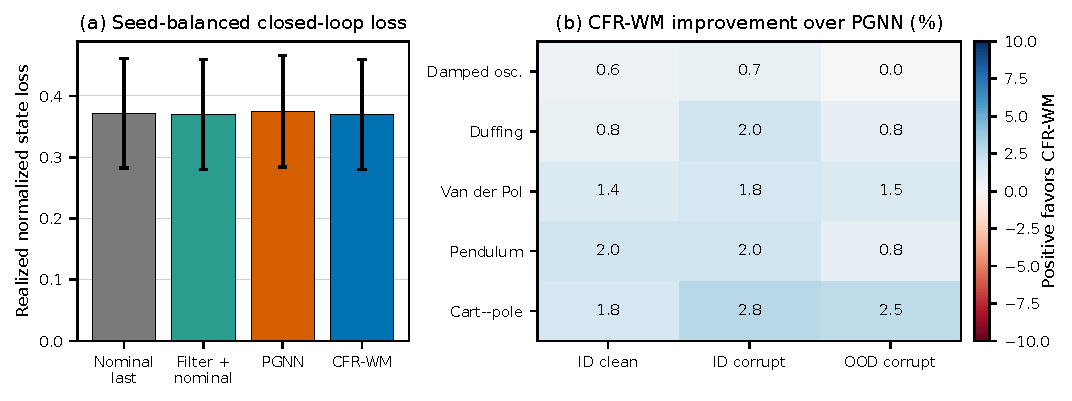
\includegraphics[width=0.94\textwidth]{figures/FigClosedLoop.pdf}
\caption{Closed-loop aggregate and heterogeneity. Error bars in (a) are SD
across eight seed-level aggregates; heat-map entries in (b) are seed means.}
\label{fig:supp-closed-loop}
\end{figure*}

\section{Measured-Flight Protocol and Full Results}

The external data set contains timestamped position, linear velocity, Euler
attitude, angular rates, and four motor commands. The reduced nominal prior
uses mass-normalized thrust, linear drag, an Euler-angle kinematic
approximation, inertia-scaled motor moments, and angular damping. The learned
residual retains the same 0.25 normalized bound used in the controlled
benchmark. Training uses only the designated training flight family;
development selects the learning rate from $\{10^{-3},3\times10^{-3}\}$ on a
separate seed. Five final seeds are then fit once. Sliding evaluation windows
do not cross flight boundaries.

Table~\ref{tab:supp-external-normalized} reports full-state NRMSE for every
method, context condition, and horizon. Table~\ref{tab:supp-external-physical}
gives position and velocity errors. The nominal prior has no training-seed
variation, so its reported SD is zero.

\begin{table*}[!t]
\centering
\caption{External full-state NRMSE, mean $\pm$ SD across training seeds after
equal weighting of the three held-out flights.}
\label{tab:supp-external-normalized}
\resizebox{\textwidth}{!}{\begin{tabular}{llrrrr}
\toprule
Context & Horizon & CFR-WM & Unfiltered & Recurrent & Nominal \\
\midrule
As recorded & 25 & $0.389 \pm 0.012$ & $0.376 \pm 0.010$ & $0.388 \pm 0.008$ & $0.488$ \\
As recorded & 50 & $0.530 \pm 0.016$ & $0.518 \pm 0.019$ & $0.519 \pm 0.006$ & $0.790$ \\
Noise & 25 & $0.393 \pm 0.012$ & $0.387 \pm 0.010$ & $0.398 \pm 0.008$ & $0.498$ \\
Noise & 50 & $0.532 \pm 0.017$ & $0.523 \pm 0.018$ & $0.527 \pm 0.006$ & $0.797$ \\
Missing & 25 & $0.397 \pm 0.011$ & $0.386 \pm 0.008$ & $0.395 \pm 0.005$ & $0.495$ \\
Missing & 50 & $0.537 \pm 0.014$ & $0.527 \pm 0.020$ & $0.526 \pm 0.007$ & $0.792$ \\
Noise + missing & 25 & $0.401 \pm 0.011$ & $0.397 \pm 0.008$ & $0.405 \pm 0.005$ & $0.506$ \\
Noise + missing & 50 & $0.540 \pm 0.014$ & $0.534 \pm 0.019$ & $0.533 \pm 0.006$ & $0.799$ \\
\bottomrule
\end{tabular}
}
\end{table*}

\begin{table*}[!t]
\centering
\caption{External position and velocity RMSE in physical units.}
\label{tab:supp-external-physical}
\resizebox{\textwidth}{!}{\begin{tabular}{lrrrr}
\toprule
& \multicolumn{2}{c}{Position RMSE (m)} & \multicolumn{2}{c}{Velocity RMSE (m/s)} \\
Context & CFR-WM & Unfiltered & CFR-WM & Unfiltered \\
\midrule
As recorded & $0.078 \pm 0.003$ & $0.083 \pm 0.010$ & $0.249 \pm 0.015$ & $0.233 \pm 0.009$ \\
Noise & $0.091 \pm 0.003$ & $0.115 \pm 0.007$ & $0.257 \pm 0.014$ & $0.258 \pm 0.007$ \\
Missing & $0.081 \pm 0.005$ & $0.095 \pm 0.022$ & $0.259 \pm 0.014$ & $0.243 \pm 0.009$ \\
Noise + missing & $0.094 \pm 0.004$ & $0.125 \pm 0.017$ & $0.267 \pm 0.014$ & $0.268 \pm 0.009$ \\
\bottomrule
\end{tabular}
}
\end{table*}

The probabilistic models use diagonal Gaussian marginals. The full external
uncertainty diagnostics are shown in Table~\ref{tab:supp-external-uncertainty}.

\begin{table*}[!t]
\centering
\caption{Measured-flight uncertainty diagnostics, averaged equally over held-
out flights and then over training seeds.}
\label{tab:supp-external-uncertainty}
\resizebox{\textwidth}{!}{\begin{tabular}{llrrrr}
\toprule
Condition & Method & NLL & Cov. & Width & Cal. error \\
\midrule
Recorded & CFR-WM & 2.264 & 0.608 & 0.453 & 0.178 \\
Recorded & Unfiltered residual & 0.794 & 0.716 & 0.526 & 0.099 \\
Noise & CFR-WM & 2.994 & 0.524 & 0.454 & 0.242 \\
Noise & Unfiltered residual & 2.361 & 0.565 & 0.528 & 0.217 \\
Missing & CFR-WM & 1.829 & 0.667 & 0.534 & 0.123 \\
Missing & Unfiltered residual & 0.735 & 0.779 & 0.685 & 0.053 \\
Combined & CFR-WM & 2.200 & 0.613 & 0.535 & 0.184 \\
Combined & Unfiltered residual & 1.130 & 0.703 & 0.688 & 0.124 \\
\bottomrule
\end{tabular}
}
\end{table*}

\begin{figure*}[!t]
\centering
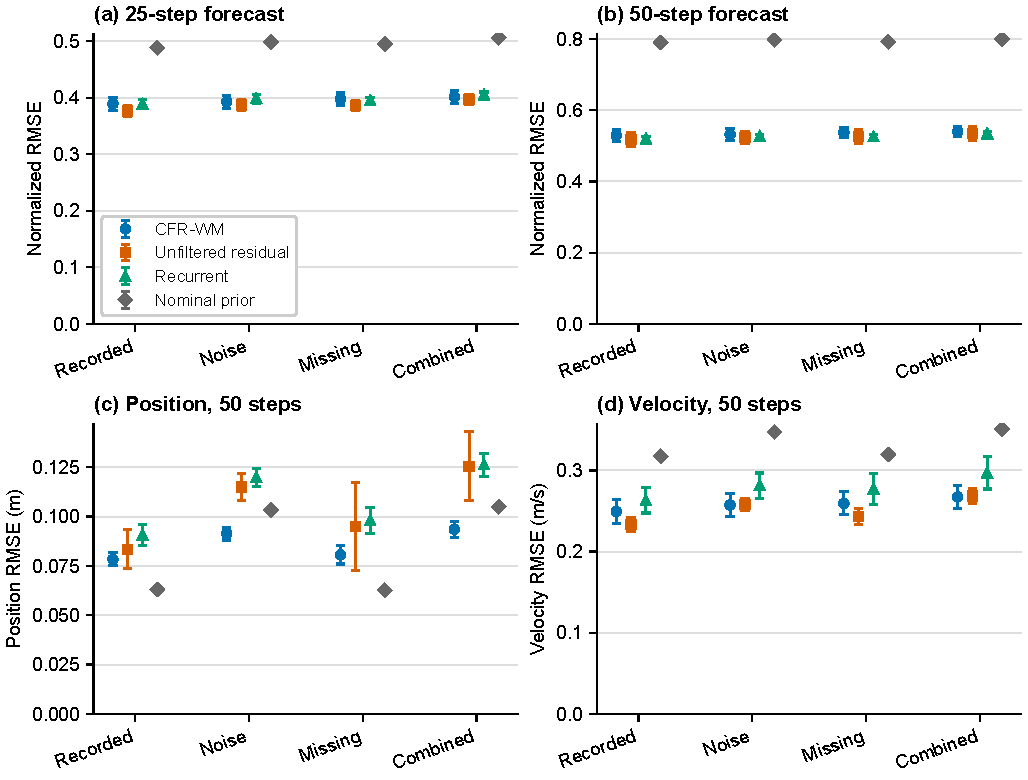
\includegraphics[width=0.94\textwidth]{figures/Fig4.pdf}
\caption{Measured-flight forecast errors by method, context condition, and
horizon. Position and full-state errors need not rank models identically.}
\label{fig:supp-external}
\end{figure*}

